\documentclass[11pt]{article}
%%%%%%%%%%%%%%%%%%%%%%%%%%%%%%%%%%%%%%%%%

\usepackage{amscd}
\usepackage{amsmath}
\usepackage{amssymb}
\usepackage{amsthm}


\usepackage{epsfig}
\usepackage{verbatim}
\usepackage{graphicx}
\usepackage{amsthm}
\usepackage{hyperref}
\pagestyle{empty}
\usepackage{color}
\usepackage[left=0.75in,top=0.35in,right=0.75in,bottom=0.35in]{geometry} % Document margins
%\usepackage[all,dvips]{xy}


\begin{comment}  

This LaTeX document is a template to be used by Bates mathematics rising seniors to create a thesis proposal. 

As a guide, the document is already filled out to represent a fictitious proposal, and all you need to do is modify the entries below to represent your own proposal.

A PDF version of the fictitious proposal is available on the department's FAQ and Policies pages, at
http://abacus.bates.edu/acad/depts/math/faq.html
and
http://abacus.bates.edu/acad/depts/math/policies.html
respectively.

Once you have finished your proposal, export it to a PDF file. Give the file a USEFUL name, for example, RiemannThesisProposal.PDF. Email the PDF file to Clementine Brasier, the 
Academic Administrative Assistant for Hathorn Hall, at cbrasier\@bates.edu

This LaTex document was created Feb/Mar 2010 by Adriana Salerno and updated Feb 2012 by Meredith Greer

\end{comment}


%\setlength{\textheight}{8.5in} \setlength{\topmargin}{0.0in}
%\setlength{\headheight}{0.0in} \setlength{\headsep}{0.0in}
%\setlength{\leftmargin}{0.0in}
%\setlength{\oddsidemargin}{0.0in}
%%\setlength{\parindent}{1pc}
%\setlength{\textwidth}{6.5in}
%%\linespread{1.6}

\newtheorem{definition}{Definition}
\newtheorem{problem}{Problem}

\newtheorem{theorem}{Theorem}[section]
\newtheorem{lemma}[theorem]{Lemma}
\newtheorem{note}[theorem]{Note}
\newtheorem{corollary}[theorem]{Corollary}
\newtheorem{prop}[theorem]{Proposition}

%%%%%%%%%%%%%%%%%%%%%%%%%%%%%%%%%%%%%%%%%

\begin{document}
	\thispagestyle{empty}
	
	
	\centerline{\textbf{\Large{Sentiment classification and usefulness prediction of Yelp reviews}}}
	
	\bigskip
	
	\noindent \textbf{Authors:} 
	Aditya Priyadarshi, Aditya Sridhar, Yogesh Gupta and Shubham Sharma
	
	\bigskip
	
	\noindent \textbf{Problem Description:} 
	The objective of this project is to train a classifier that classifies the user given reviews in natural language into positive or negative categories for various restaurants in the Yelp dataset \cite{yelp}. In addition, we are also planning to undertake the task to determine whether any particular user review can be categorized as useful or not.
	
	\bigskip 
	
	\noindent \textbf{Summary of Data:} 
	The original dataset described in the Yelp Dataset Challenge 9 \cite{yelp} has 4.1M reviews and 947K tips by 1M users for 144K businesses spread across four cities. We are planning to use a subset of the given data. In our initial experiments, we have taken first 5000 reviews. The anonymized data is provided in JSON format for each review and each user profile. In the initial set of 5000, we had no missing data. Each individual review data consists of anonymized IDs for the business, user and review, star rating, review type, review text and votes on how useful, funny or cool the review is. The relevant variables in the user data consists of review count, the number of fans, the number of useful, funny, cool votes the user’s reviews have received in addition to other attributes.
	\begin{figure}[h]
		\centering
		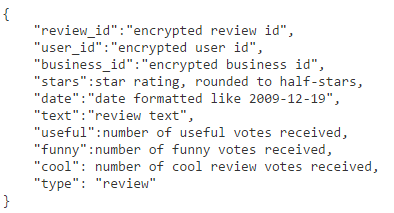
\includegraphics[]{data_format.png}
		\caption{Review Data Format}
	\end{figure}
	
	
	\bigskip
	
	\noindent\textbf{Methods:}
	We plan to use Naive Bayes and SVM to train our classifier as discussed in paper \cite{plv} using bag-of-words feature. In addition, we also intent to use convolutional neural networks (CNN) and recurrent neural networks (RNN) as discussed in papers \cite{kim} and \cite{ydlb} respectively using word2vec feature.
	\bigskip
	
	\noindent\textbf{Preliminary results:}
	In our initial experiment, we tried Naive Bayes classifier for sentiment classification using Python. We took first 5000 reviews in the dataset and divided into training set (80\%) and validation set (20\%). Reviews with star rating of 3,4 and 5 were considered positive and 1,2 as negative. We have then selected 6790 words from selected corpus as bag-of-words features which have term frequency of five or more and document frequency of two or more. Naive Bayes implementation provided by NLTK was used for training classifier. On the validation set, we have received an accuracy of 77.8\% using Naive Bayes for sentiment classification into positive and negative reviews.
	\bigskip
	
	\begin{thebibliography}{9}
		% NOTE: change the "9" above to "99" if you have MORE THAN 10 references.
		
		\bibitem{yelp} Yelp Dataset Challenge \url{https://www.yelp.com/dataset_challenge}
		\bibitem{plv} Bo Pang, Lillian Lee and Shivakumar Vaithyanathan. \textit{Thumbs up? Sentiment Classification using Machine Learning
			Techniques}, In EMNLP, 2002.   
		
		\bibitem{kim} Yoon Kim. \textit{Convolutional Neural Networks for Sentence Classification}, In EMNLP, 2014.
		
		\bibitem{ydlb} Dani Yogatama, Chris Dyer, Wang Ling, Phil Blunsom. \textit{Generative and Discriminative Text Classification
			with Recurrent Neural Networks}, arXiv preprint arXiv:1703.01898, 2017
		
	\end{thebibliography}
	
	%%%%%%%%%%%%%%%%%%%%%%%%%%%%%%%%%%%%%%%%%
	
	
	
	
	
	
\end{document} 
